\subsection{Simulated TCEs}
\label{s:simulated}
In order to measure the performance of the Robovetter and the \Kepler\ Pipeline, we created simulated transits, simulated false positives, and simulated false alarms. In statistical parlance, this was done to quantify the type I errors (the number of times we incorrectly allow false alarms into our list of candidates) and type II errors (the number of times we did not fail known false positives).  The simulated transits are created by injecting transit signals into the pixels of the original data. The simulated false positives were created by injecting eclipsing binary signals and positionally off-target transit signals into the pixels of the original data (see \citealt{Coughlin2017a} and \citealt{Christiansen2017} for more information). The simulated false alarms were created in two separate ways: by inverting the light curves, and by scrambling the sequence of cadences in the time series. The TCEs that resulted from these simulated data are available at the Exoplanet Archive on the Kepler simulated data page.\footnote{\label{kepsimpagefn}\url{https://exoplanetarchive.ipac.caltech.edu/docs/KeplerSimulated.html}}

%For both the \invtce{s} and the \scrtce{s} we needed to remove true astrophysical events, as explained in \S\ref{s:clean} below, in order to match the false alarms found in the \opstce data set.
%JLC1: I think the final sentence is confusing extra detail in the intro paragraph to this section. % SEM Agreed.

\subsubsection{True Transits -- Injection}
\label{injectsec}

We empirically measure the completeness of the \Kepler\ Pipeline and the subsequent vetting by injecting a suite of simulated transiting planet signals into the calibrated pixel data and observing their recovery, as was done for previous versions of the \Kepler{} Pipeline \citep{Christiansen2013a,Christiansen2015,Christiansen2016}. The full analysis of the DR25 injections are described in detail in \citet{Christiansen2017}. In order to understand the completeness of the Robovetter, we use the on-target injections \citep[Group 1 in][]{Christiansen2017}; we briefly describe their properties here. For each of the \ninjecttargs{} targets, we generate a model transit signal using the \citet{Mandel2002} formulation, with parameters drawn from the following uniform distributions: orbital periods from 0.5--500 days (0.5--100 days for M dwarf targets), planet radii from 0.25--7 \re{} (0.25--4 \re{} for M dwarf targets), and impact parameters from 0--1. After some re-distribution in planet radius to ensure sufficient coverage where the \Kepler{} Pipeline is fully incomplete (0\% recovery) to fully complete (100\% recovery), 50\% of the injections have planet radii below 2\,\re{} and 90\% below 40\,\re{}. The signals are injected into the calibrated pixels, and then processed through the remaining components of the \Kepler{} Pipeline in an identical fashion to the original data. Any detected signals are subjected to the same scrutiny by the Pipeline and the Robovetter as the original data. By measuring the fraction of injections that were successfully recovered by the Pipeline and called a planet candidate by the Robovetter with any given set of parameters (e.g., orbital period and planet radius), we can then correct the number of candidates found with those parameters to the number that are truly present in the data. While the observed population of true transiting planets is heavily concentrated towards short periods, we chose the 0.5--500 day uniform period distribution of injections because more long-period, low signal-to-noise transits are both not recovered and not vetted correctly --- injecting more of these hard-to-find, long-period planets ensures that we can measure the Pipeline and Robovetter completeness. In this paper we use the set of on-target, injected planets that were recovered by the \Kepler{} Pipeline (the \injtce{s}, whose period distribution is shown in Figure~\ref{f:simtces}) to measure the performance of the Robovetter. Accurate measurement of the Robovetter performance is limited to those types of transits injected and recovered.

{\color{blue}It is worth noting that the injections do not completely emulate all astrophysical variations produced by a planet transiting a star.  For instance, the injected model includes limb-darkening, but not the occultation of stellar pulsations or granulation, which has been shown to cause a small, but non-negligible, error source on measured transit depth \citep{Chiavassa2017} for high signal-to-noise transits.  }


\subsubsection{False Alarms -- Inverted and Scrambled} 

To create realistic false alarms that have noise properties similar to our \opstce{s}, we inverted the light curves (i.e., multiplied the normalized, mean-zeroed flux values by negative one) before searching for transit signals. Because the pipeline is only looking for transit-like (negative) dips in the light curve, the true exoplanet transits should no longer be found. However, quasi-sinusoidal signals due to instrumental noise, contact and near-contact binaries, and stellar variability can still create detections. In order for inversion to exactly reproduce the false alarm population, the false alarms would need to be perfectly symmetric (in shape and frequency) under flux inversion, which is not true. For example, stellar oscillations and star spots are not sine waves and SPSDs will not appear the same under inversion. However, the rolling band noise that is significant on many of \Kepler's channels is mostly symmetric.  The period distribution of these \invtce{s} is shown in Figure~\ref{f:simtces}. The distribution qualitatively emulates those seen in the \opstce{s}; however there are only $\sim$60\% as many.  This is because the population does not include the exoplanets nor the eclipsing binaries, but it is also because many of the sources of false alarms are not symmetric under inversion.  The one-year spike is clearly seen, but is not as large as we might expect, likely because the broad long-period hump present in the DR25 \opstce{} distribution is missing from the \invtce{} distribution. We explore the similarity of the \invtce{s} to \opstce{s} in more detail in \S\ref{s:simularity}.

Another method to create false alarms is to scramble the order of the data. The requirement is to scramble the data enough to lose the coherency of the binary stars and exoplanet transits, but to keep the coherency of the instrumental and stellar noise that plagues the \Kepler\ data set. Our final solution was to scramble the data in coherent chunks of one year. The fourth year of data (Q13--Q16) was moved to the start of the light curve, followed by the third year (Q9--Q12), then the second (Q5--Q8), and finally the first (Q1--Q4). Q17 remained at the end. Within each year, the order of the data did not change. Notice that in this configuration each quarter remains in the correct \Kepler\ season preserving the yearly artifacts produced by the spacecraft. 

Two additional scrambling runs of the data, with different scrambling orders than described above, were performed and run through the \Kepler{} pipeline and Robovetter, but are not discussed in this paper, as they were produced after the analysis for this paper was complete. These runs could be very useful in improving the reliability measurements of the DR25 catalog --- see \citealt{Coughlin2017a} for information.


\begin{figure*}[hp]
 \begin{center}
  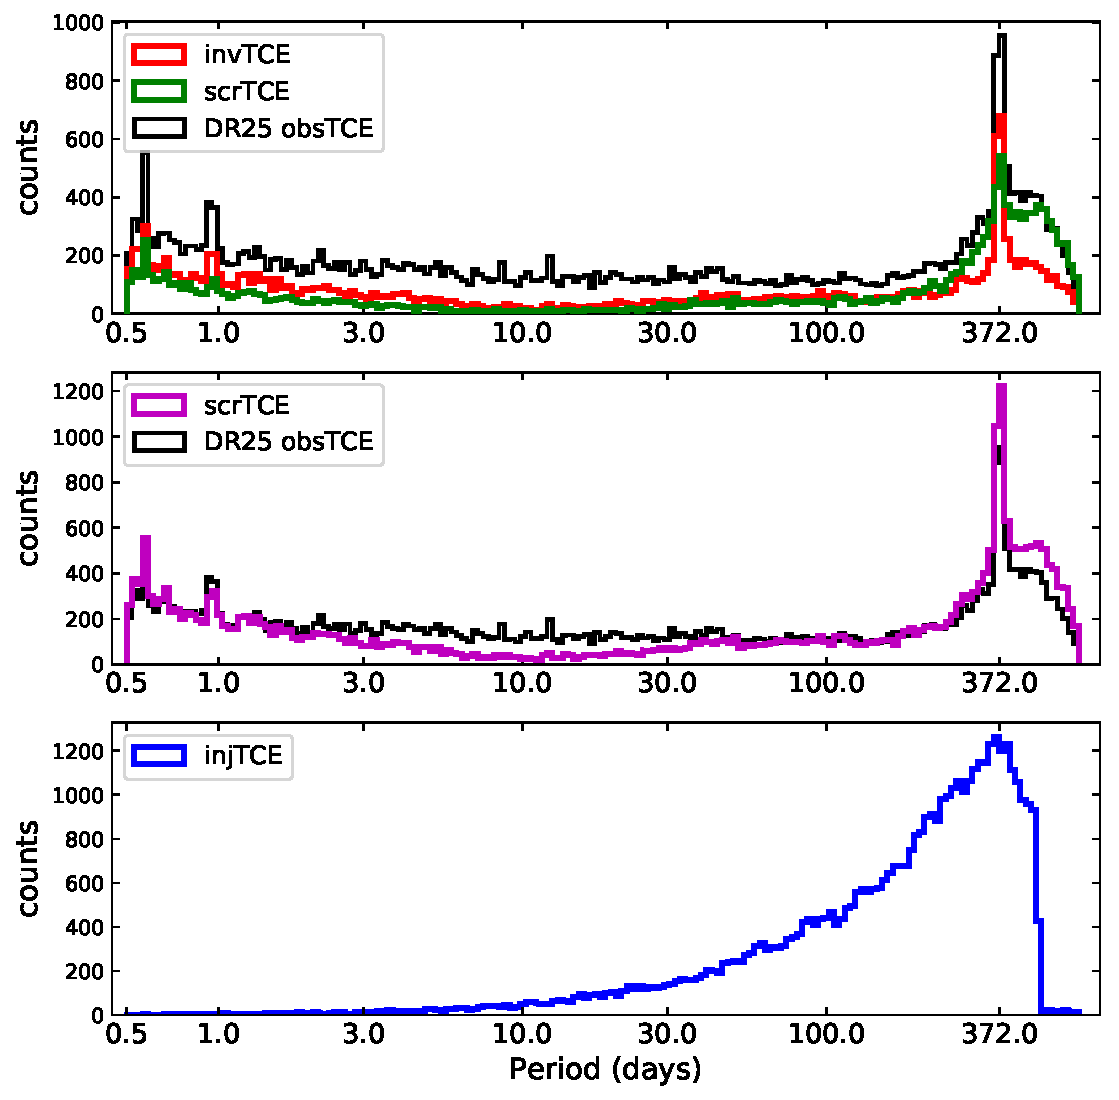
\includegraphics[width=\linewidth]{f2.pdf}
  \caption{Histogram of the period in days of the cleaned \invtce{s} (top, red), the cleaned \scrtce{s} (middle, green), and \injtce{s} (bottom, blue) in uniform, base-ten logarithmic spacing. The DR25 \opstce{s} are shown for comparison on the top two figures in black.  At shorter periods ($< 30$\,days), the difference between the simulated false alarm sets and the observed data represents the number of transit-like KOIs; at longer periods we primarily expect false alarms. Notice that the \invtce{s} do a better job of reproducing the one-year spike, but the \scrtce{s} better reproduce the long-period hump. Because the \injtce{s} are dominated by long-period events (significantly more long-period events were injected), we are better able to measure the Robovetter completeness for long-period planets than short-period planets.}
  \label{f:simtces} 
 \end{center}
 \end{figure*}



\subsubsection{Cleaning Inversion and Scrambling}
\label{s:clean}
As will be described in \S\ref{s:relcalc}, we want to use the \invtce\ and \scrtce\ sets to measure the reliability of the DR25 catalog against instrumental and stellar noise. In order to do that well, we need to remove signals found in these sets that are not typical of those in our \opstce\ set. For inversion, there are astrophysical events that look similar to an inverted eclipse, for example the self-lensing binary star, KOI~3278.01 \citep{Kruse2014}, and Heartbeat binaries \citep{Thompson2012}. With the assistance of published systems and early runs of the Robovetter, we identified any \invtce\ that could be one of these types of astrophysical events; 54 systems were identified in total. Also, the shoulders of inverted eclipsing binary stars and high signal-to-noise KOIs are found by the Pipeline, but are not the type of false alarm we were trying to reproduce, since they have no corresponding false alarm in the original, un-inverted light curves. We remove any \invtce{s} that were found on stars that had 1) one of the identified astrophysical events, 2) a detached eclipsing binary listed in \citet{Kirk2016} with morphology values larger than 0.6, or 3) a known KOI.  After cleaning, we are left with \ninvtces\ \invtce{s}; their distribution is plotted in the top of Figure~\ref{f:simtces}.

For the scrambled data, we do not have to worry about the astrophysical events that emulate inverted transits, but we do have to worry about triggering on true transits that have been rearranged to line up with noise. For this reason we remove from the \scrtce\ population all that were found on a star with a known eclipsing binary \citep{Kirk2016}, or on an identified KOI.  The result is \nscrtces\ \scrtce s; their distribution is plotted in the middle panel of Figure~\ref{f:simtces}. 
{\color{blue}This will not remove all possible sources of astrophysical transits. Systems with only two transits (which would not be made into KOIs), or systems with single transits from several orbiting bodies would not be identified in this way. For example, KIC~3542116 was identified by \citet{Rappaport2017} as a star with possible exocomets, and it is a \scrtce\ dispositioned as an FP.  But we expect the effect of not removing these unusual events to be negligible on our reliability measurements relative to other systematic differences between the \opstce{s} and the \scrtce{s}.
}
%Or, astrophysical events similar to the mysterious dips on KIC~8462852 ("Boyajian's Star") \citep{Boyajian2016} could create \scrtce{s} (the \scrtce{s} does not include KIC~8462852.)

After cleaning the \invtce{s} and \scrtce{s}, the number of \scrtce{s} at periods longer than 200\,d closely matches the size and shape of the \opstce{} distribution, except for the one-year spike. The one-year spike is well represented by the \invtce{s}.  Combining the two sets appears to give a good handle on the type and relative frequency of false alarms present in the DR25 \opstce\ population. Tables\,\ref{t:invclean} and \ref{t:scrclean} lists those \invtce{s} and \scrtce{s} that we used when calculating the false alarm effectiveness and false alarm reliability of the planet candidates.

\begin{deluxetable}{lrrc}
\tablecolumns{4}
\tablewidth{\linewidth}
\tabletypesize{\scriptsize}
\tablecaption{\invtce{s} used in the analysis of catalog reliability}
\label{t:invclean}
\tablehead{
\colhead{TCE-ID} & \colhead{Period} & \colhead{MES} & \colhead{Disposition}\\
\colhead{(KIC-pn)} & \colhead{days} &  &\colhead{PC/FP}\\
}
\startdata
000892667-01 &    2.261809 &       7.911006 &   FP \\
000892667-02 &  155.733356 &      10.087069 &   FP \\
000892667-03 &  114.542735 &       9.612742 &   FP \\
000892667-04 &  144.397127 &       8.998353 &   FP \\
000892667-05 &   84.142047 &       7.590044 &   FP \\
000893209-01 &  424.745158 &       9.106225 &   FP \\
001026133-01 &    1.346275 &      10.224972 &   FP \\
001026294-01 &    0.779676 &       8.503883 &   FP \\
001160891-01 &    0.940485 &      12.176910 &   FP \\
001160891-02 &    0.940446 &      13.552523 &   FP \\
001162150-01 &    1.130533 &      11.090898 &   FP \\
001162150-02 &    0.833482 &       8.282225 &   FP \\
001162150-03 &    8.114960 &      11.956621 &   FP \\
001162150-04 &    7.074370 &      14.518677 &   FP \\
001162150-05 &    5.966962 &      16.252800 &   FP \\


\tablecomments{This table is published in its entirety in the machine-readable format. A portion is shown here for guidance regarding its form and content.}
\end{deluxetable}

\begin{deluxetable}{lrrc}
\tablecolumns{4}
\tablewidth{\linewidth}
\tabletypesize{\scriptsize}
\tablecaption{\scrtce{s} used in the analysis of catalog reliability}
\label{t:invclean}
\tablehead{
\colhead{TCE-ID} & \colhead{Period} & \colhead{MES} & \colhead{Disposition}\\
\colhead{(KIC-pn)} & \colhead{days} &  &\colhead{PC/FP}\\
}
\startdata
000757099-01 &    0.725365 &     8.832907 &   FP \\
000892376-01 &  317.579997 &    11.805184 &   FP \\
000892376-02 &    1.532301 &    11.532692 &   FP \\
000892376-03 &  193.684366 &    14.835271 &   FP \\
000892376-04 &  432.870540 &    11.373951 &   FP \\
000892376-05 &  267.093312 &    10.308785 &   FP \\
000892376-06 &    1.531632 &    10.454597 &   FP \\
000893004-01 &  399.722285 &     7.240176 &   FP \\
000893507-02 &  504.629640 &    15.434824 &   FP \\
000893507-03 &  308.546946 &    12.190248 &   FP \\
000893507-04 &  549.804329 &    12.712417 &   FP \\
000893507-05 &  207.349237 &    11.017911 &   FP \\
000893647-01 &  527.190559 &    13.424537 &   FP \\
000893647-02 &  558.164884 &    13.531707 &   FP \\
000893647-03 &  360.260977 &     9.600089 &   FP \\


\tablecomments{This table is published in its entirety in the machine-readable format. A portion is shown here for guidance regarding its form and content.}
\end{deluxetable}
